% Put labels, etc., on figures using PSTricks.
% Use dvips -E <file>.dvi -o <file>.eps to create encapsulated PostScript.
%
\documentclass[12pt]{article}
\usepackage{graphicx}
\usepackage{pstricks}
\pagestyle{empty}

\begin{document}
\rput(5,-5){
\rput(.1,-.1){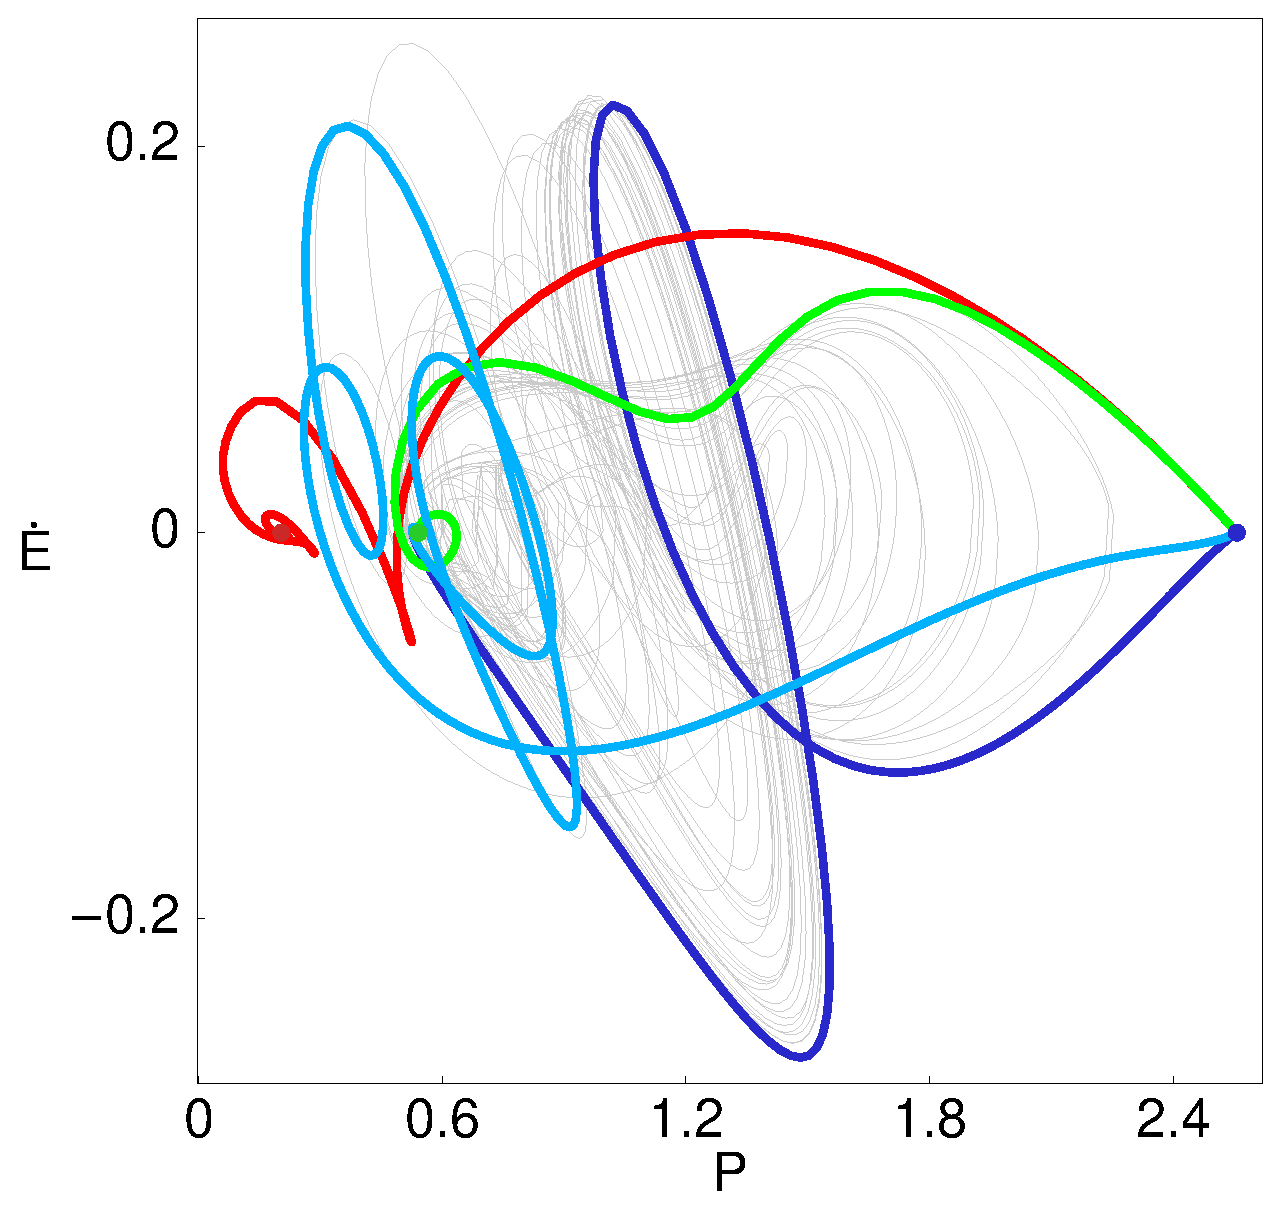
\includegraphics{../../figs/connPEdot.eps}}

\huge

% \psframe*[linecolor=white](-6.5,6)(-5.5,7)
% \psframe*[linecolor=white](6,-6.5)(7.2,-5.5)

\rput(10.1,2.2){E$_3$} 

\rput(-6,0.4){E$_1$}

\psline[linewidth=2pt]{->}(-4.8,-1.65)(-3.8,1)\rput(-5.3,-1.55){E$_2$}
\psline[linewidth=2pt]{->}(4.5,-5)(2,-2.7)\rput(6.5,-5.5){``Turbulence''}


% Use grid command below to place objects at specified coordinates.
%   \psgrid[subgriddiv=1,griddots=10](-8,-8)(10,10)
}
\end{document}
